\documentclass[12pt]{report}
\usepackage[utf8]{inputenc}
\usepackage[T1]{fontenc}
\usepackage[english]{babel}
\linespread{1.50}

\usepackage{geometry}
 \geometry{
 a4paper,
 total={170mm,257mm},
 left=30mm,
 right=30mm,
 top=20mm,
 bottom=30mm,
 }

%%% Bibliography
\usepackage[square,numbers]{natbib}
\usepackage{url}
\usepackage{hyperref}
\bibliographystyle{abbrvnat}


%%% Grafik
\usepackage{epstopdf}
\usepackage{graphicx}
\usepackage{float}

%%% math
\usepackage{amsmath}
\usepackage{amsfonts}
\usepackage{amssymb}
\usepackage[amssymb]{SIunits}
\usepackage{units}
%%% Kode
\usepackage{listings}

%%% TABLES
\usepackage{tabularx}
\usepackage{booktabs}

%%% Farve formaterring 
\usepackage{color}

%%% Dokument miljø 

\title{Package delivery}
\author{Group A325}
\date{October-December 2018}

\begin{document}

\maketitle

\tableofcontents




\chapter{Introduction}
In a forward moving world, online shopping is steadily growing. The puzzle of getting packages delivered is constantly getting more important. There are a lot of options to make an optimal package delivery route for all parts of the system, both the recipient of the package and the delivery company. A route which considers the fuel economy of the route and ensures that a truck does not have to return to a street more than once and ensures the convenience of the recipient. Thereby satisfying all parts of the transaction. \\\hspace*{5 mm}
All delivery firms have their own methods of optimization but the optimal mathematical solution to delivery routes is yet to be found\cite{notsolved}. Therefore package delivery keeps being problematic which leads to our initial problem.


\section{The initial problem}
In this section the initial problem is presented and it will be the foundation for this report. The initial problem consists of one main question and [REPLACE ME] sub questions to which will be answered in order to narrow down the problem field. \\

There are many different problems in package delivery that could be improved upon. But there seems to be a general interest in improving customer satisfaction. It would therefor be interesting to investigate how to optimize the delivery system in a way that would benefit the end customer.

\textbf{Main question:} How can package delivery be optimized to insure better customer satisfaction? \\

\textbf{Sub questions:} \\
\begin{itemize}
\item What are the correlation between package delivery and online shopping?
\item Who uses online shopping?
\item What are important for the customer?
\item Which existing methods are there to optimize routes?

\item How do existing methods solve the problem?
\item 
\end{itemize}




\chapter{Problem analysis}
Package delivery is a large industry and can be optimized in many ways. It would therefore be interesting to see if there is any specific problems in the industry that would benefit a large portion of the delivery companies if optimized. To be able to find these specific problems we need to determine the scale and growth of this industry and look at the top delivery companies to determine what methods they are using to improve customer satisfaction. \\\hspace*{5 mm}
Our main focus is to satisfy the end customer and improve on their customer experience while still having a focus point in the companies interests. Looking at what customers value will give a suggestion to what is relevant to look into. One of the important aspects of package delivery are the preferred delivery methods and why people prefer different package methods. Then we can determine what delivery method we are interested in optimizing and how that would be possible. Here it would be interesting to look at what affects delivery time and how to optimize routes with algorithms.


\section{The increase in online shopping}
The increased popularity of the internet has made it more accessible for people to order packages from all over the world. In 2017, a total of 176 million e-commerce where made which is an increase of 9\% compared to 2016. 135 million of these trades involved physical products that in some way needed shipping.\cite{FDIHyearreport}. In 2017, 80\% of Danes have used online shopping within the last year, When it only was 59\% in 2008. \cite{Ehandel2017} \\\hspace*{5 mm}
The growth in package delivery are sure to continue and the need for optimization are increasing. The leading delivery companies have a large and complex logistic challenge that is constantly evolving.\cite{notsolved}
\\\hspace*{5 mm}
There have been a shift over the last three years on how the customers want to have their packages delivered. 2017 was the first year where "collect yourself" is more popular than delivering to your home address \cite{FDIHyearreport}. There are multiple factors that could have impacted this change. Most prominently the introduction of a new kind of pick-up points called parcel lockers or boxes, which is unmanned places in public areas. The customer can pick up the package using a personal code sent to the customer. This makes it more convenient for the customers to collect their packages. \\

\section{Customer Convenience}
With the increase in online shopping, we see delivery companies more often in our day to day lives. For these companies it is a constant competition to keep the customers.
Within the package delivery business the main focus for the customers is the shortest possible time and the most convenient delivery. In an attempt to make it more convenient for the customers PostNord have a function called "Modtagerflex", this is for the customer to give their permission to place the package in a predetermined place, this requires a spot that is hidden. PostNord releases itself for the responsibility when the package is signed out of their system. This means if it gets stolen while standing on the spot determined, it is no longer PostNord that has any ties with the package, this means that your own insurance company would be the one covering. But in most insurances it says it has to be locked inside the house. which is hardly the case when PostNord needs acces to the place to put the package.http://nyheder.tv2.dk/2017-05-07-frustrerede-postnord-kunder-venter-forgaeves-buddet-lyver-om-at-i-har-forsoegt-at midlertidig kilde her\\\hspace*{5 mm}
In a survey sent out by us on various social media sites, we asked a various of questions about package delivery. One hundred participants answered the survey. They were mainly under the age of 26, and the vast majority have had a package delivered within the last year.

Customers who gets home delivery are often frustrated by the fact they stay home the whole day, and still it is not certain that the package will be delivered at the house. Most companies are very unspecific with the delivery time, for example does Post Nord only give the day it will be delivered, which means that you would have to take a whole day at home, for you to make sure you are there when the package gets delivered.
%Customers who wants delivery to their doorstep are often frustrated by the large time period in which the package are set to arrive. Most package delivery companies are very unspecific when it comes to the period of time where the customers need to be home. For example does PostNord only tell you the estimated day of arrival and not any specific time frame. Therefore in this case the unspecific delivery interval means people will have to take the whole day off to receive their packages.

Customers who wants delivery to their doorstep are often frustrated by mailmen who say they have tried to deliver your package when they in fact have not. People who ordered home delivery now have to go pick it up at a pick up point.

\begin{figure}[H]
  \centering
  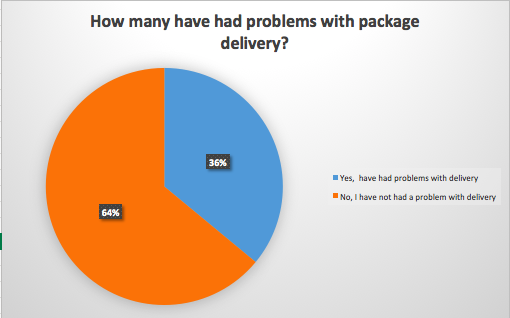
\includegraphics[width=200]{pics/problemswithpackage.png}
  \caption{Problems with a package}
  \label{fig: Customer satisfaction}
\end{figure}

In a survey which we conducted, we asked one hundred people different questions about their experience with package delivery in which 36\% have had problems within the last year. While this is not the majority it still is a significant number of people in which have had a problem with a service that you have to pay for.\\\hspace*{5 mm}
And while it is 36\% that have had a problem in which they themselves define it, a more significant number have had a package delivered while they were not home, this is described and showed in the next graph.
\begin{figure}[H]
  \centering
  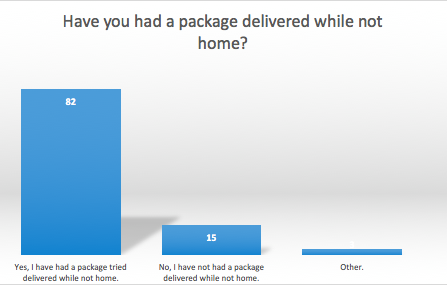
\includegraphics[width=300]{pics/packagedeliverednothome.png}
  \caption{Package delivered while not at home}
  \label{fig: Customer satisfaction}
\end{figure}

 83\% of the participants in our survey have experienced that while they were at work a delivery company have attempted to deliver a package to their house. This becomes a problem for not only the customer that has to agree upon a new delivery date or pick up the package at a pick-up point. And the delivery company has spend time driving to a customer that is not available, which means they have spend resources on a delivery that might have to happen again at a later date.

\begin{figure}[H]
  \centering
  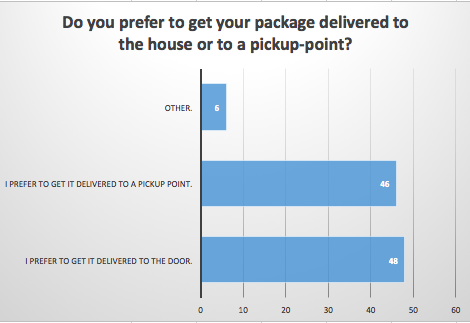
\includegraphics[width=300]{pics/houseorpickuppoint.png}
  \caption{Do you prefer house or pick-up point.}
  \label{fig: Customer satisfaction}
\end{figure}

In our survey the preferred way to get a package delivery is close to evenly split. With a 46\% preferring to pickup the package at a shop or other package pick-up points. While 48\% prefer to get it delivered to their home. 
This is often reasoned to the point that they are never home when the package is getting delivered and it would be easier for them to pick it up on the way to or from work or class.


\begin{figure}[H]
  \centering
  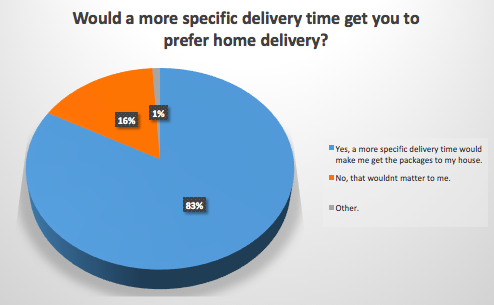
\includegraphics[width=300]{pics/morespecific.png}
  \caption{Would a more specific time help with being home.}
  \label{fig: Customer satisfaction}
\end{figure}

 With a narrower time frame the delivery companies could make sure people are home when a package delivery is attempted. Because the receiver only have to be home for maybe an hour or two instead of a whole day.\\\hspace*{5 mm}
 83 \% of people would rather have their package delivered to their doorstep if they could choose a time frame of the day. \\

The hundred people asked in our survey would mostly want their package delivered home, if the possibility for a stricter time frame or even being a part of picking the time themselves. This could solve problems for both parties of package delivery. The customers would have a bigger chance of being home when their package was getting delivered, and the delivering companies would not have to make as many drives to people whom are not home. 



\section{Frequent users of online shopping}
We have already established that the amount of people who purchases online is gradually increasing every year. This section focuses on the different age groups that use the internet for shopping.

\begin{figure}[H]
  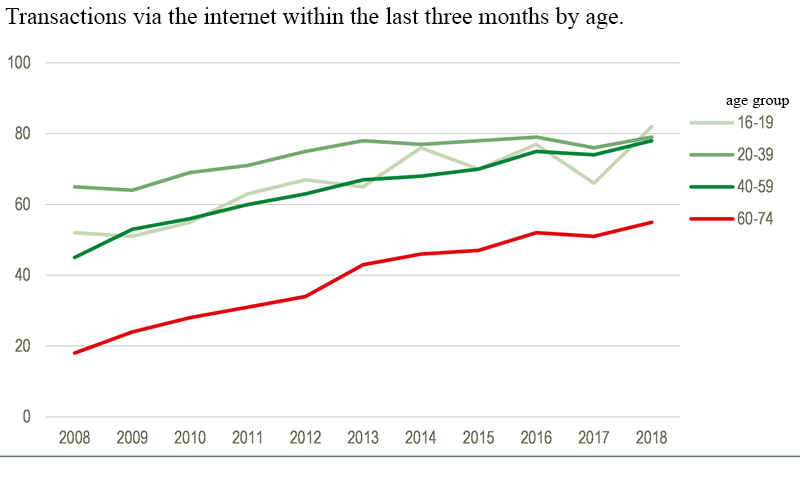
\includegraphics[width=\linewidth]{pics/customer.png}
  \caption{Age groups over time. \cite{danmarkstat2}}
  \label{fig:Age groups over time}
\end{figure}

A statistic from 2018 show that 82\% of people in Denmark between ages 16 and 19 have been online shopping within the last 3 months. While the age groups from 20 to 39 years and 40 to 59 years sits at 79\% and 78\% respectively, see figure 2.1. 55\% of elders between 60 and 74 years have used online shopping in last three months which may seem like a small amount compared to the younger age groups, but the elders have increased their online shopping more than any other age group. In 2008 they was only at 18\% which conclude an increase of 37\% within the last 10 years \cite{danmarkstat1}.
While the statistics does not show a big difference in the the two younger age groups covering ages 16 to 59, it does show that younger people tend use the internet for shopping more frequently. \\
Where a customer chooses to get their package delivered is highly affected by their age. Younger people tend to use the pick-up points more often while the older age groups prefers home delivery.\cite{FDIHyearreport}. \\



\section{Satisfaction and returning customers}
Costumer satisfactory is often high on the priority list of companies and having satisfied customers often results in returning customers\cite{FDIHyearreport}. As part of this problem analysis we conducted a survey mentioned in section 2.2. The survey show that 36\% of our participants have experienced some kind of problems within the last year. \\\hspace*{5 mm}
FDIH made a study on what factors is important for returning customers in correlation to online shopping. The four factors in this study is credibility, relevance, responsiveness and convenience. These factors are weighted as a way to compare importance in correlation to the customer return rate. The weight of each factors are based on a survey that was answered by more than 14 thousand danish customers in 2017. The NPS score on the right of figure 2.6 indicates the correlation to promotors and detractors.

\begin{figure}[H]
  \centering
  \includegraphics[width=300]{pics/Satisfaction.png}
  \caption{Customer satisfaction. \cite{FDIHyearreport}}
  \label{fig: Customer satisfaction}
\end{figure}

Package delivery is part of responsiveness and convenience which the study shows are the most prominent factors \cite{FDIHyearreport}. If the customer is not satisfied with the delivery time/methods it would often result in them using a different online shop next time they shop online. We established that more than a third had experienced problem with their package delivery so companies that have online shops have a big interest in optimizing the package delivery to satisfy their customers which result in returning customers. This means that both online-shop companies and the end customer would benefit from optimization in package delivery.



\section{Top delivery companies and their methods}
The Danish package distribution is being handled by a lot of different companies with some being more known than others. PostNord and GLS are by far the most known and used companies. A research involving 2323 private citizens, 506 companies and 212 public institutions showed that 90 \% mentioned PostNord when asked to mention post distributors in Denmark. GLS is mentioned by 69 \% of the participants while lesser known distributors as DHL Express and UPS is mentioned by roughly 25\% of the participants in the research\cite{reportDKpakketjenester}. \\\hspace*{5 mm}
Receiving mail is an everyday phenomenon. Getting packages delivered to either a home address or a parcel box on a weekly basis is getting more common. In the research mentioned earlier in this section, one in four people receive packages ordered online up to three times a month and around two thirds receives one or more packages every quarter of the year. How these people choose to get their packages delivered varies depending on their place of residence. People living in bigger cities shows a tendency to receive packages more frequently than ruralites \cite{reportDKpakketjenester}. Getting packages delivered to home addresses is still the most used method by city residents and ruralites. Most cities offers other alternatives such as parcels boxes, which stores the package for you to pick up, while rural areas are more reliant on home deliveries due to longer travel time to the nearest pick-up point.\cite{reportDKpakketjenester}.\\\hspace*{5 mm}
Parcel boxes are getting used more. Usage have risen 10 \% from 2015 to 2018 while delivery to home addresses have fallen 7 \% in the same time period. Elderly people above the age of 65 is more likely to use home delivery while the younger age groups and families with children are more frequently users of the parcels boxes and pick up points\cite{FDIHyearreport}.

Postnord and GLS both provide their own solutions to comprehend the delivery requirements giving by the customers, but their solution only provide the customers with influence by some degree. Both PostNord and GLS provide a service that let the customer choose where on their address that the distributor is allowed to put it. This gives the customer the freedom of not needing to be home at the time of delivery but also presents a problem. The customer is held fully responsible if the package is either lost or stolen from their address after it has been delivered by the distributor\cite{postnordoptions}\cite{glsoptions}. Furthermore this service is not optimal if living in an apartment complex where no secluded areas are available for the package to be placed. As mentioned earlier, parcels boxes is widely used by the danish population and both PostNord and GLS delivers to these while also being able to drop the package of at a pick up point either chosen by the customer or closest in proximity if nothing has been specified by the customer\cite{postnordoptions}\cite{glsoptions}.

In all the cases of delivery options giving by the distributor described above, none of them gives the customer full control of the delivery time. They provide solutions that involves the customer in risking losing their package\cite{Pakketyveri} GLS even provides the customer with the option of what day they want the package delivered, but this still forces the customer to be at home at the time of delivery if they want the package without risking it being stolen if placed somewhere on the address\cite{Pakketyveri}.



\section{Last Mile Delivery}
Last mile delivery is a logistics term and refers to the final step of the order being dispatched from a transportation hub to the customer receiving their package.

Last mile delivery has become a problem for couriers as this part of the delivery process is often less efficient than transporting goods via container ships or trucks. The increase in e-commerce has also contributed to this problem, as people are buying more products online and demand fast shipping times. Increased e-commerce means more packages being sent, and couriers are now searching for new ways to transport goods as traditional transportation methods aren't successful anymore. \\\hspace*{5 mm}


New transportation technologies are being developed to help lower the cost and increasing the efficiency of last mile delivery \cite{FastForwardingLast-mileDelivery}. Companies are looking to drones, droids, and autonomous delivery vehicles. By using semi and fully autonomous delivery vehicles in cities couriers will be able to reduce delivery costs by 10 to 40 \% while also reducing their CO2 emissions greatly by using electric vehicles. \\

\section{Impact of traffic related instances}

Delivery companies often have problems specifying the time in which costumers receive their packages that results in them only telling you a specific day. A big reason to this is the uncertainty when it comes to traffic. We have investigated when the traffic peaks on a couple of central Aalborgs big roads. As we assume these central roads in the inner city will have a great impact on the delivery times. 

We have examined the six streets Karolinelundsvej, Kastetvej, Sohngårdsholmsvej, Vesterbro, Østerbro, and Østre Alle \cite{traficcount}. And have concluded that the traffic congestion on these streets follow the work hours in Denmark. The beginning peak time on all six streets in the morning are 07:23 on average, this is when people start their commute to work. And the beginning of the peak time in the afternoon are 15:05 on average which is close to peoples commute from their work to their home. 

Thereby we can conclude that the most optimal time of the day to deliver packages, are in the hours between 8 in the morning and 15 in the afternoon, which is when people are at work. But as we have seen in our user survey, people choose to get their packages delivered to a package pickup point. Because they might not be home in these hours, therefore the most convenient and efficient time of day for the delivery company, would be before peak hours in the morning, or after peak hours in the afternoon. Nonetheless the delivery companies will have to take the peak hours into consideration. As they can greatly impact the delivery time estimate if not calculated for. 



\section{The economy}
\subsection{Postnord}
Postnord have had a downfall from 2016 to 2017 in their net revenue on 1.4 mio SEK . 
In the same period Postnord have also managed to get smaller (driftomkostninger), which is a probability, because they are getting bigger competition from the other package delivery companies, like GLS, UPS and so on. 
Also, their EBIT made had a large decrease from 2015 (564 Mio SEK) to 2016 (-1083 Mio SEK)  and then the EBIT had an increase to 2017 (-124 Mio SEK), which is an increase on 959 Mio SEK.
Even though Postnord are getting more competition on the marked by other package delivery companies, they are delivering even more packages than before, as you can see from the yearly rapports about the concern. But still they deliver less mail and less B-post and C- post, this is one of the reason they are having a smaller net revenue. 
PostNord often forms part of a long and complex supply chain, in which collaboration with suppliers is core. The suppliers that PostNord engages for road transportation are in many cases small workers like trucks and employees. PostNord suppliers also include large, well-established operators in areas such as IT, staffing, air transport and rail transport. Postnord is using a lot of resources to make their deliveries greener, and healthier for the environment. the specific requirements for road transportation is important for Postnord to see that their drivers are holding the rules, both on drive/resting time, and the laws in the different countries they are driving through. 

After 1. January 2017 SKAT removed the special rules for E-business companies usage of the taxation law 
Which means that ordering things from the internet, will be cheaper, and is therefore a win for the industries, both the package delivery industry, and the E-business. And because there were no tax obligations on the “Postal Offices” delivering of packages, since 1989, they have had big advantages, in package delivery since they could deliver their packages cheaper than the other package delivery companies.   

\subsection{GLS}

\section{UPS Orion}


\section{Algorithm}
The package delivery problem is basically a variation of the travelling sales man problem. The travelling salesman problem evolves around a salesman, who have to visit n number of cities, and then return home to his own town. The best solution to for his route is therefore a Hamiltonian route where he only visits every city once before he travels home to the starting point. \\ \\
The travelling salesman problem is a well known problem in computer science and especially graph theory because it is known to be NP-complete. As it is a multigraph where there usually are at least two ways to get to the next city. And therefore there will be at least two edges to every vertice.\cite{tsp} 

\begin{figure}[H]
  \centering
  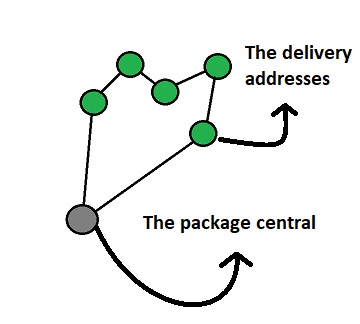
\includegraphics[width=300]{pics/tsp.jpg}
  \caption{The Travelling Salesman Problem}
  \label{fig: The Travelling Salesman Problem}
\end{figure}\textbf{}

This is also the issue in the delivery problem, as there in most cases will be more than one way to reach each address. An example of this can be seen in Figure 2.7 which is an example where the delivery driver needs to travel from the package central to 5 different delivery addresses. In the delivery problem version of the travelling salesman problem it will be the route where the delivery truck does not have to visit or cross a street more than once\cite{tsp}. There has not been found an algorithm which can solve the problem, the best solution for the problem. Was created by Keld Helsgaun from Roskilde University\cite{keld} who created an algorithm which makes a route that is only 0.0474 percent longer than optimal route\cite{tsp2}. Each delivery company therefore have different computer programs and algorithms they use. Even businesses who only focus on package routing have been started, an example of this is Routific who has created a piece of software they sell to companies who needs routing for delivery\cite{routific}.         


\subsection{Genetic algorithm}
The idea behind genetic algorithm comes from Charles Darwin's theory of evolution and is based on the survival of the fittest principal. The algorithm therefore uses that the strongest element in the generation gets to be the father for the next generation. To solve the problem of package delivery you start with a generation of random routes. Each of the routes gets assigned a fitness value depending on how close it is to the goal that is the best route/shortest route. The route with the best score gets to be the father of the next generation of routes. This selection keeps happening until the best route have been discovered or made. Or at least until the fitness score gets balanced and does not improve further in the next generations\cite{geneticalg}.

\subsection{Greedy algorithm}
There is no known algorithm that solves TSP fast enough. Therefore there have surfaced algorithms to make the best possible solution in a certain amount of time. The greedy algorithm is one, it always takes the nearest city which has not been visited, this creates the most direct route between the cities, this creates the best solution locally and expects the result on a larger scale to be close to the optimized solution. While this outcome is a faster route than a random picked route, it is not in all cases the most optimized route.\cite{solvingcdp} 

\chapter{Afgrænsning}

\chapter{Problemformulering}

Draft // The delivery period for the customers are too big. \\
Can be solved with a piece of software that can optimize package delivery so that the customer has a better idea of when the packages will arrive at their doorstep.



\bibliography{kilder}


\end{document} 